\documentclass[10pt,a4paper]{article}
\usepackage[utf8]{inputenc}
\usepackage{amsmath}
\usepackage{amsfonts}
\usepackage{amssymb}
\usepackage{graphicx}
\usepackage{hyperref}
\usepackage{float}
\usepackage[left=3cm,right=3cm,top=3cm,bottom=3cm]{geometry}
\usepackage{listings}

\lstset{
   basicstyle=\footnotesize\ttfamily,
   tabsize=2,
   breaklines=true
}

\author{Nicholas Shindler}
\title{people tracking and prediction \\ \large Kalman Filter \& LSTM Neural Network Prediction}

\begin{document}
\maketitle

\bigskip 

\tableofcontents

\vspace*{\fill}
\begin{abstract}
This project explores the analysis of human motion. focusing primarily on short term motion prediction using probabilistic and machine learning approaches and comparing the results. This project covers tracking multiple people. Data is designed to be collected by RGB-d camera. A basic Kalman Filter is used for prediction. A simple RNN utilizing LSTM is also examined for prediction.
\end{abstract}
\vspace*{\fill}


\section{Introduction}
In this report I will cover, the intended goals of the project, the general structure of the project, how I tested the effectiveness of my algorithms, and discuss how I met my goals and the results of my tests. In this project I combing machine learning and probabilistic methods to predict human motion. I use the ATC pedestrian tracking data-set for my people data, as it allowed me both the ability to test my system with a large number of people being tracked at the same time, and a large amount of available data to train my motion prediction neural network. My goal was to evaluate real time prediction and compare a probabilistic to machine learning approach, as well as combine both approaches for hopefully the best results. I constructed this project to run in real time, and operate both with minimal data as well as a robust and fault tolerant structure.

\section{Project Goals}
This project is designed to evaluate the effectiveness of prediction of human motion. The core component of this project is a prediction module that uses a Kalman Filter with a basic motion model to predict tracks of people. A secondary aspect of the project was a detection node to convert data from rgb-d video (read in as point clouds) to people tracks. This was set to be done with the Point Cloud Library (pcl) and a SVM algorithm for ground plane based people detection. Additionally I wanted to experiment with the comparison of results between a probabilistic approach and a machine learning approach to people detection, using an LSTM neural network to predict motion with similar data input to the kalman filter. and then combine both methods to see if they could achieve even better results.

\section{Application: design and design choices}
This project was done using the robotic operating system (ROS) as the basic framework. This allowed the different tasks to be broken into sections based on task (detection, prediction, etc). Google Colab was also leveraged for training the neural network. Additionally the ATC pedestrian tracking data-set was leveraged heavily (\url{https://irc.atr.jp/crest2010_HRI/ATC_dataset/}).

\subsection{Camera and data input}
Because this project was done with Ubuntu 18/ROS Melodic, the ROS bridge for the Kinect 2 would not run, and a Kinect 1 camera was used. The data from the Kinect camera was brought in using the \textit{openni} package. This data was represented in the ROS \textit{PointCloud2} format.

\subsection{Detection}
The \textbf{Point Cloud Library (pcl)} was going to be leveraged in conjunction with a pre-configured SVM for people detection. However, due to issues with the code supplied by the tutorial, and project priorities, a pseudo detector was created the used the \textbf{ATC pedestrian tracking data-set} for a data stream and published the data to a ros topic in the same format as if it was begin taken from real time video. This method ended up giving a number of advantages. Most significantly it provided data with multiple people tracks and a variety of motion patterns. however as a  result, the detector for live data was never completed.

The data both from the camera and from the ATC tracks, read in data at a rate of 30 readings/frames a second. The detector was setup to use a buffer system allowing a variable rate of data publishing based on the needs of other modules in the system. I set it up to publish data at \~10/second.

\subsection{Prediction}
The prediction module had 2 main parts. At an interval of 10/second data was read in and passed into a full Kalman Filter utilizing both the prediction and update steps. A second part ran at a rate of 1/second that would create a prediction vector for each of the people tracks at that stage. These predictions used the prediction stage of the Kalman Filer, and recorded a prediction every second for 8 seconds into the future. This prediction was enhanced, by using the prediction from the previous time interval to update the prediction. This worked where the prediction at time $t$, $n$ seconds into the future would take the prediction at time $t-1$, at $n+1$ seconds and run the \textit{update} section of the Kalman filter with both values. this was done for the first 7 ($n-1$) predictions, as the final ($n^{th}$) prediction had no previous time interval prediction, and therefore only used the \textit{prediction} section of the Kalman filter. These updates also used the same Kalman Filter instance as the filtering of the data, which should cause the quality of the update to improve the longer the tracks were analyzed. 

The Kalman Filter used a basic motion model based on constant velocity motion:
\begin{equation}
x_{n+1} = x_n + \dot{x_n}*\Delta t
\end{equation}
\begin{equation}
y_{n+1} = y_n + \dot{y_n}*\Delta t
\end{equation}

\subsection{Evaluation}
While the data detection and prediction modules operate in real time. The Evaluation module runs at the end of a data collection interval. The collection interval is configured to run for 30 seconds. The data is recorded in seconds an millimeters. The evaluation stage creates 2 data-sets. One data set is printed as a human readable log, and an example of this is included at the end of this report. this data set tracks the error for each person and prediction interval, with averages done over time. The second data set is setup to be create plots using \textbf{gnuplot}. There are gnuplot scripts for graphing in the data module of the project. This data uses the position and trajectory error at each time interval and prediction step, averaged over all people tracks in each time frame. I also found plotting tracks of the data and predictions provided a good visual indication of the results being achieved.

\subsection{Neural Network}
Using the ATC data a neural network was created and trained on google colab. this NN used a basic LSTM structure, predicting a person's state at the next timestep using the previous second's worth of recording data. while better results could be achieved by expanding the model, I felt it was important to keep the data being input to a similar time interval as what the Kalman Filter was using. Particularly as I hoped to feed the prediction for the NN into the KF, to create a \textit{deep kalman filter}, which I felt would give the best results for motion prediction.

The Neural network was trained on a separate data set from the one being used by the detection module as pseudo detection tracks. I used a subset of 2500000 elements for training the model.

I exported the model into my project to be utilized by a python ROS node, that could return predictions based on inputs passed by a ROS service call from the prediction node.

While I am limiting myself to 1 second of data for what I am passing into the model, this has a vast number of permutations in terms of structure. The data input is structured to contain a history size (the basic block of previous data input), a batch size (breaking the data into repeated sections), and a step (this is simplify to just be 1). The input data needed is equal to the history size plus the batch size. For me this will be limited to 10 so it can be implemented in the prediction algorithm. my goal was to set up the integration into ROS so that multiple similar models could be tested.


\section{Experimentation Results}

\subsection{Probabilistic Prediction}
\begin{center}
\textit{the first note is that if you are looking at the code that creates the evaluation data, it is not constructed, efficiently, it is not ordered logically, it was written to minimize the amount of data being read into memory at any given time.}

\textit{the second note is that I am presenting this data as data, without trying to say if this is good/bad error, or an acceptable deviation, or any other value based judgments. this is because I have collected and analyzed this data without a \textit{goal}, in so much as I I am not doing anything with the predictions. Depending on the application the numbers \textit{mean} wildly different things. As people prediction for a robot moving in a crowded shopping mall will need a much higher resolution of prediction ($\pm0.1$ meter), than a drone that needs to have an idea where all the people will be by the time it's missile hits the ground ($\pm3$ meters).}
\end{center}
 
\subsubsection{sorting through the data}

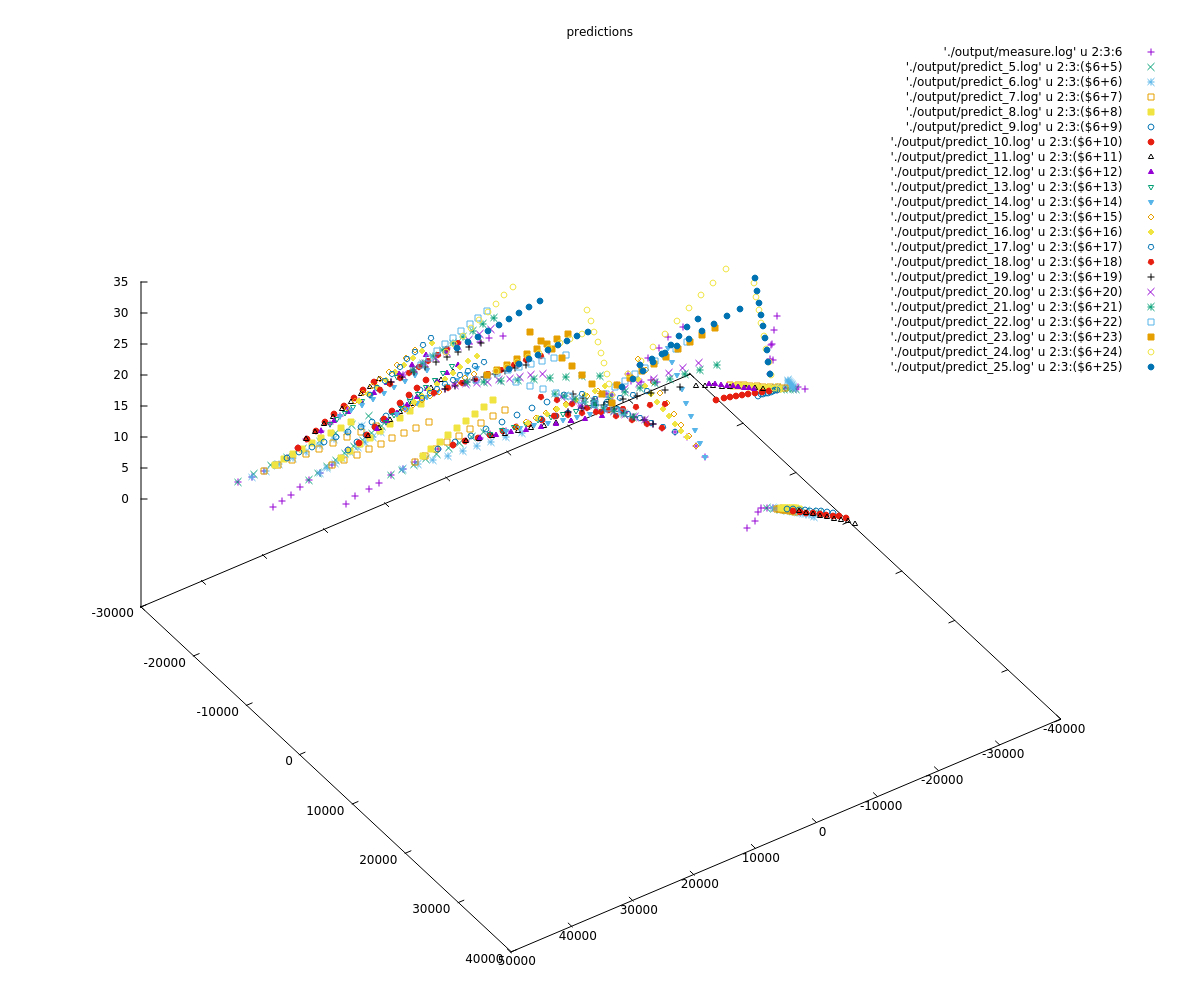
\includegraphics[width=\textwidth]{../graphs/prediction_data.png}\\

My decisions about how to represent this data focus on the idea of representing the error, and how it changes, rather than trying to present \textbf{all} the data.

with that in mind I have provided an examination of the data tracks for a visual error approximation, as well as calculations of how the error changes numerically over time.

\subsubsection{people tracks}
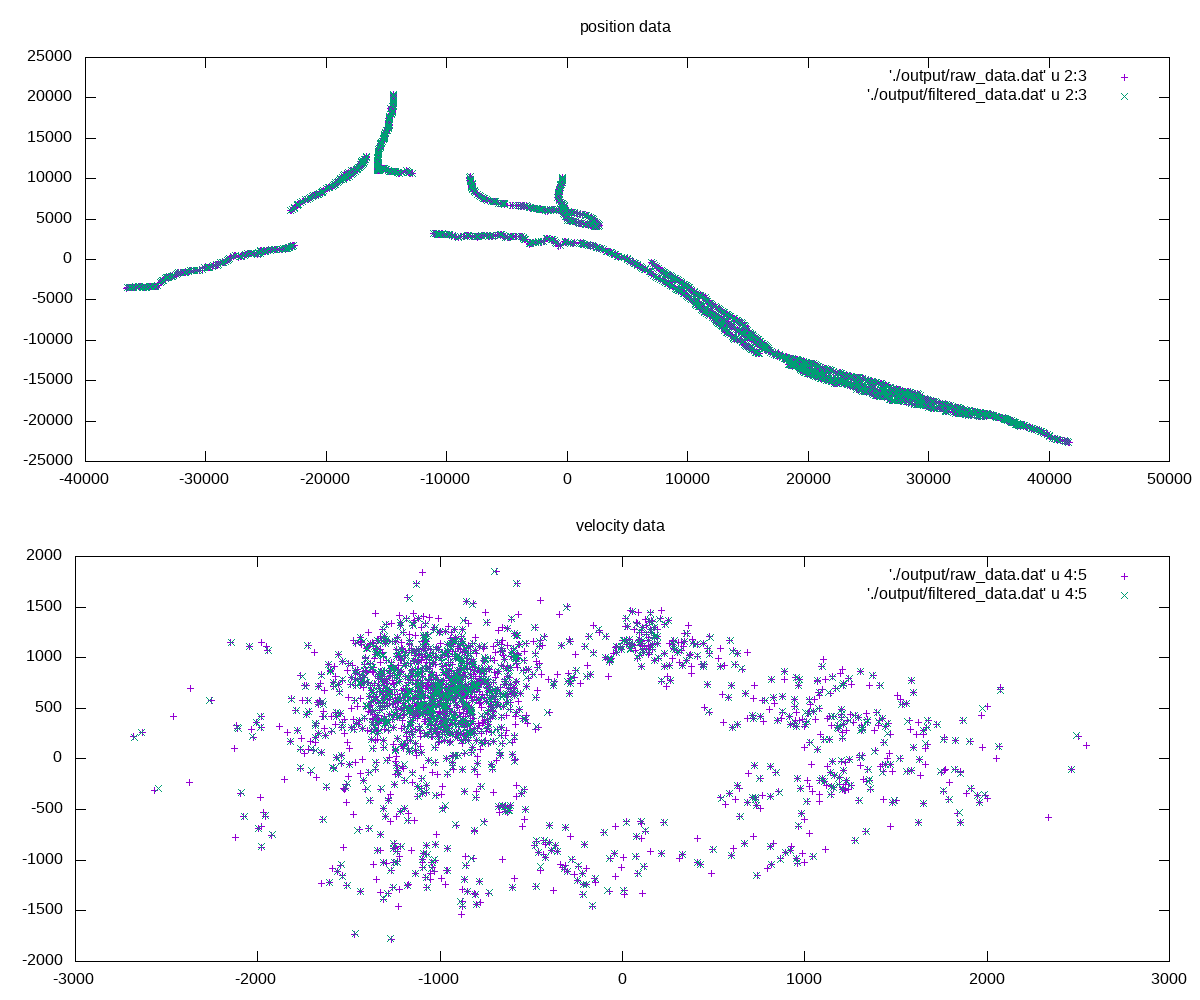
\includegraphics[width=\textwidth]{../graphs/raw_data.png}\\

this is a basic plot of what the data looks like. As you can see the distribution of the velocity is not incredibly meaningful by itself, however it does give a good idea of how the Kalman Filter (filtered data) changes the raw data, something not as visible in the position, displaying the failing of the motion model to account for changes in velocity, particularly at higher speeds. the velocity plot also does well to show the direction of motion for the people as a group.

The position tracks show the people motion on the x y plane. As you see most of it is relatively linear. However there are also many short segments representing potentially people that the detector lost track of for some time. As well as non-linear tracks.

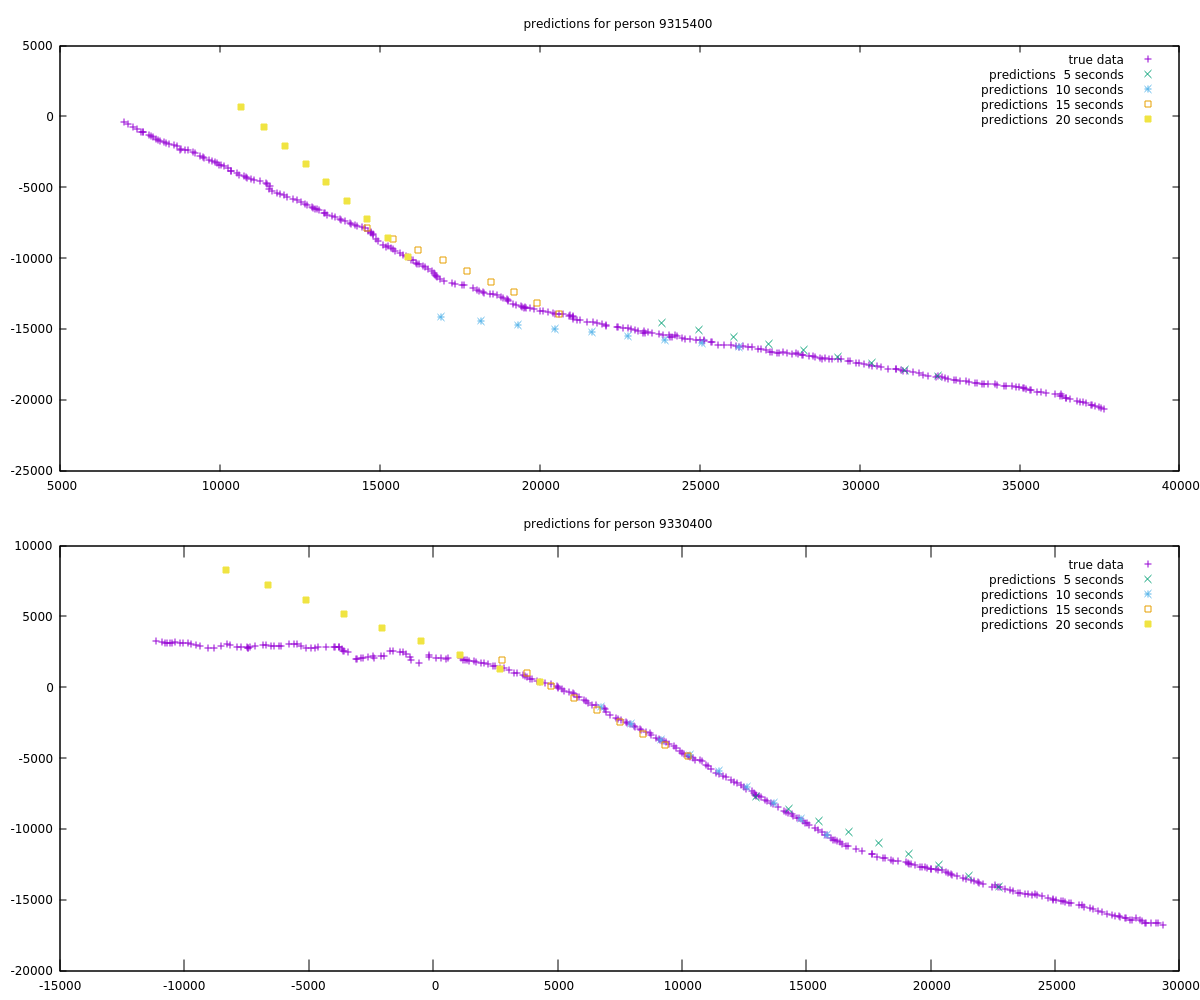
\includegraphics[width=\textwidth]{../graphs/person_tracks.png}\\
These two people tracks were chosen for the most part because they are 2 of the longest continuous tracks. In these tracks you can see both were the predictions succeed and when they fail. the predictions at 15 and 10 seconds of person $9330400$'s track are very good, over the entire 8 seconds, however, as soon as there is a change in trajectory like at 20 seconds, the prediction quickly gets very bad.

\subsubsection{error over time}
\textit{there are small x-axis offsets to the data this is artificial to allow all the data to be easily read on the same graph. in reality all data occurs on 1 second intervals.}

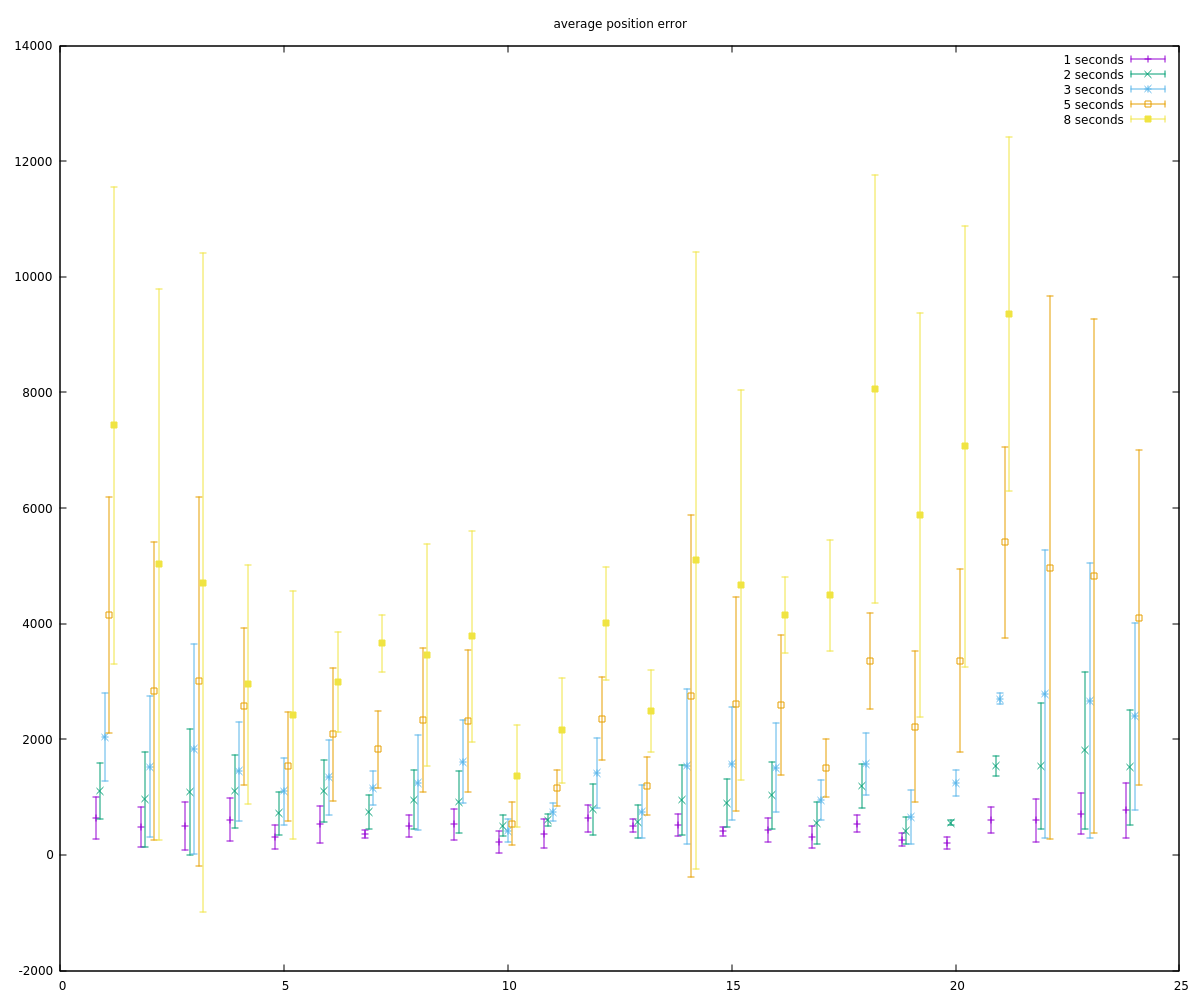
\includegraphics[width=\textwidth]{../graphs/average_position_error.png}\\
this error is the calculated absolute positional error, averaged over each person on the time interval, and point is plotted for 5 of the 8 prediction intervals, the error bars are based on the standard deviation. The error is calculated as the absolute distance between the measured and predicted points on the x y plane. I was surprised that there did not appear to be any improvement in prediction over time, based on the Kalman Filter updating it's values. I think that this was because the changing amount of people and in the system, and the similarity of real tracks to the model, effected the data so much more than the accuracy of the KF. I also found it notable that at the longer prediction intervals the deviation grew substantially, demonstrating once again the limitations of the model being used.
 
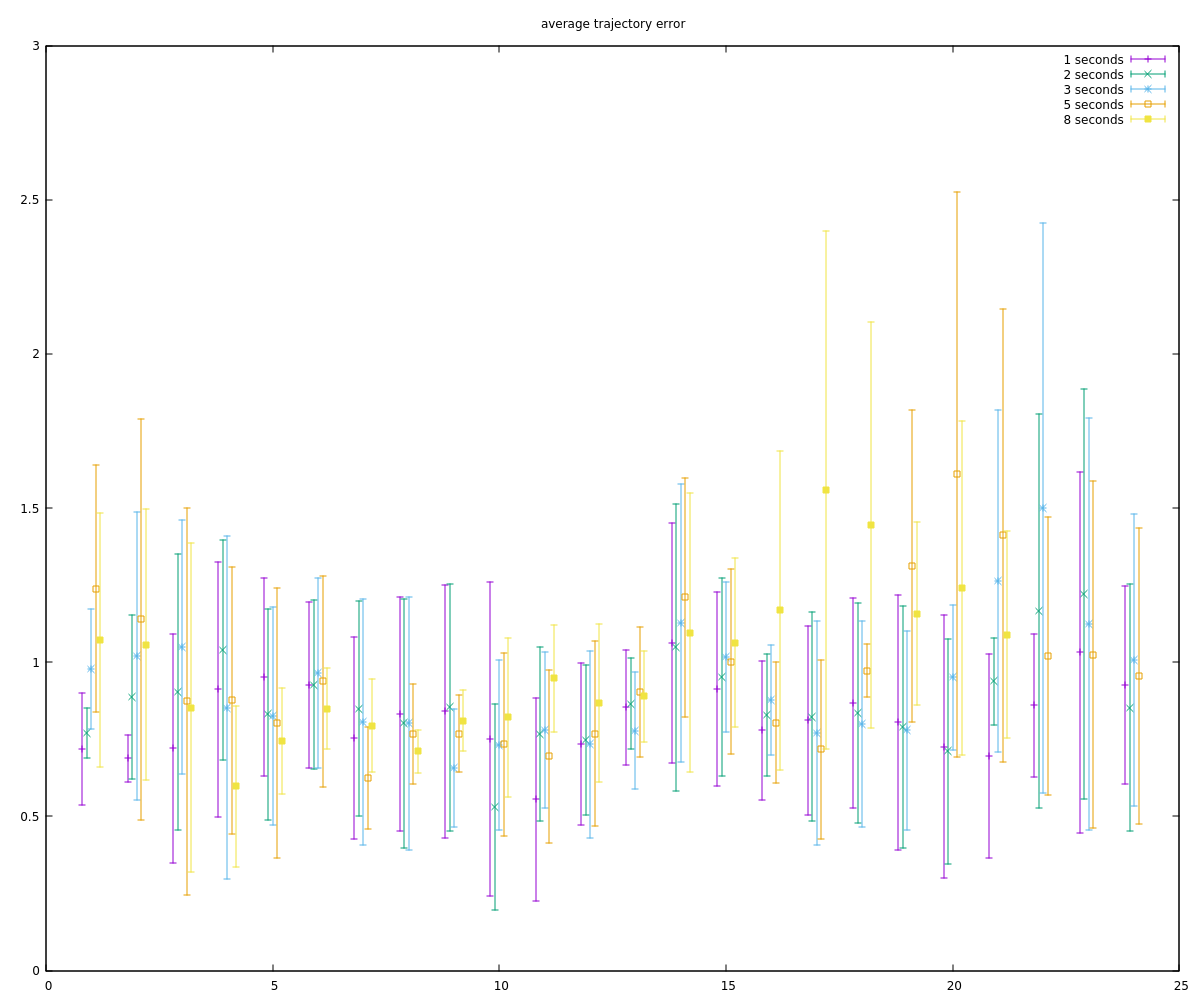
\includegraphics[width=\textwidth]{../graphs/average_trajectory_error.png}\\
This data was constructed similarly to the position data in the previous section, however, the error is calculated as the angle between the predicted and measured velocity vectors. From the way that the trajectory error is relatively constant over both trial time and prediction time, we can see a reinforcement that some tracks \textit{follow} the model, traveling in a straight line, and have a rather low trajectory error, while other tracks turn, or curve, creating consistently wrong trajectories that do not get either better or worse over time.

\subsection{Machine Learning Prediction}
Due to the ML model not being fully integrated into the ROS infrastructure, live testing has not yet happened. However basic analysis of the models was done during training.
\subsubsection{the model}
training the model required iterative testing to determine the optimum format for the data, particularly the ability to run it in a real time process. This means I was not able to set a long history length for example as I these predictions are iterative and short term, requiring small amounts of data. Particularly as most single motion tracks are less than 10 seconds. Therefore I chose to use a 1 second interval for history, requiring the 10 previous readings. Additionally, I worked to get a good relationship between the size of the data set I was using for training, and the fitting interval length and epoch number. training over 15 epochs of length 1250, with 150 validation steps, and 2500000 data points, I think I have a well trained model.
\begin{figure}[H]
\caption{Training and validation loss} 
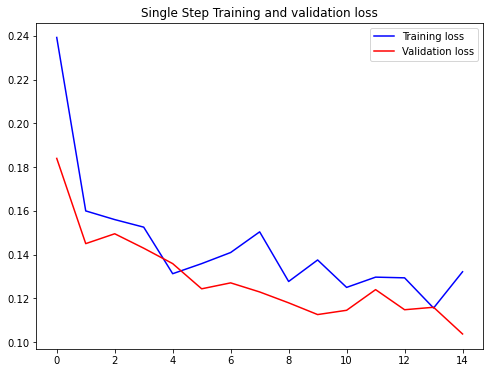
\includegraphics[width=\textwidth]{../graphs/training_loss.png}
\end{figure}
\subsubsection{the predictions}
While I didn't want to duplicate work, by creating a complex evaluation program in Colab, as part of the training evaluation I picked out graphs for people tracks.
\begin{figure}[H]
\caption{x and y position prediction} 
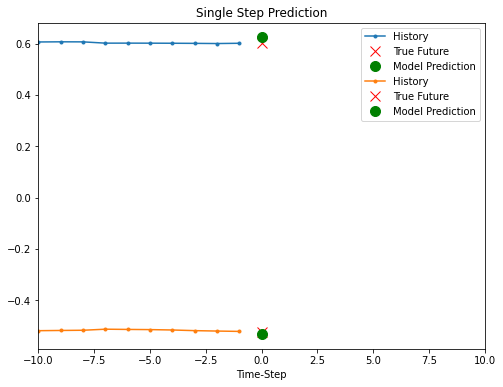
\includegraphics[width=0.5\textwidth]{../graphs/xy_val_one.png}
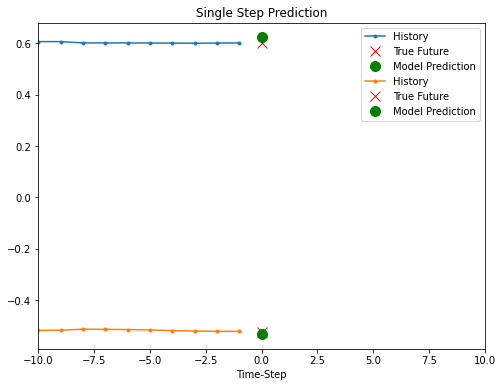
\includegraphics[width=0.5\textwidth]{../graphs/xy_val_two.png}
\end{figure}

\begin{figure}[H]
\caption{linear velocity prediction} 
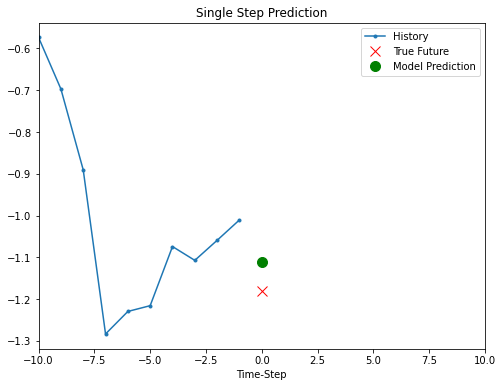
\includegraphics[width=0.5\textwidth]{../graphs/vel_val_one.png}
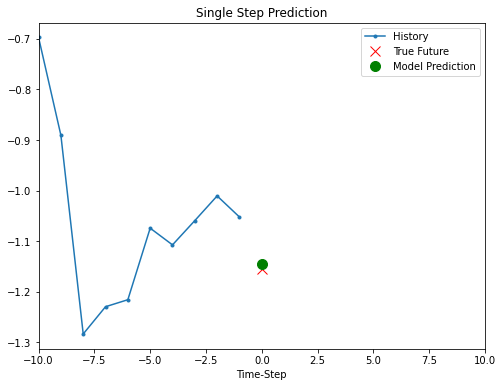
\includegraphics[width=0.5\textwidth]{../graphs/vel_val_two.png}
\end{figure}
I found that the velocity predictions were significantly less accurate than the position predictions, they generally offered a substantial improvement over the KF model (that was constant velocity). 

However the predictions were much more erratic in terms of the rotational velocity and orientation. Which are understandably harder to predict. 
\begin{figure}[H]
\caption{angular velocity prediction} 
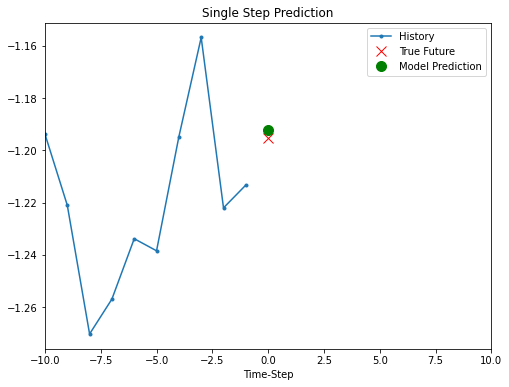
\includegraphics[width=0.5\textwidth]{../graphs/th_val_one.png}
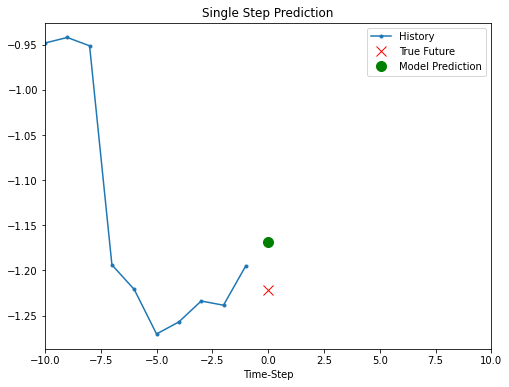
\includegraphics[width=0.5\textwidth]{../graphs/th_val_two.png}
\end{figure}
I think that use in combination with a Kalman Filter would smooth the variation here and provide better average results.

\subsection{System Robustness}
I have tested this system with up to 20 people being tracked at the same time. While it was able to handle the relatively large volume of people, I do not thing it can handle many more. Thinking about this, while I have in place a number of safeguards for the data input failure, I should have placed a maximum value to the people being tracked to prevent a memory overload. This is probably the largest area of vulnerability in the system as it is currently constructed. 

I am very happy with the system's ability to handle a large data load. a number of design choices make sure to prevent memory overflow. Particularly the data is read in on a line by line basis, therefore the 1.0 gb data file does not actually have to be loaded, only 1 line at a time is in memory. Similarly the prediction data is written to log files making the theoretical limit on trial length (how long you can collect predictions) set by disk space and input data rather then RAM. Also by using the ROS framework I have been able to use the built in parallelism in ROS to make the code run more efficiently, particularly when adding in additional prediction methods. Making it so detection, probabilistic prediction, and neural network prediction can all run on separate threads, but share data.

\section{Discussion}

\subsection{goals completed}
While I had hoped to be able to achieve both I found building a Machine Learning algorithm for prediction more interesting of a challenge particularly as I had access to a large data set of people tracks. This was coupled with the fact there did not appear to be any simple configuration for creating a people detection model with RGB-d data only models that use normal video, making the depth aspect of the camera less important. Therefore I did not end up completing the detection, in favor of exploring using machine learning for prediction. 

My prediction integration with the NN was also not completed at the time of this writing, however I am hoping to have it implemented.

I was able to complete all aspects of my probabilistic prediction goals. 

\subsection{method effectiveness}
I found it it surprising that a simple model for motion would yield such good results. In general the effectiveness of the predictions depended entirely on if a person turned. While walking in a direction without turning the predictions even out to 8 seconds often performed quite well, it was only in instances when a person would change direction or drastically change velocity that a prediction would nearly immediately loose all bearing on reality.

It was my hope that the inclusion of predictions from the neural network would help with the issues related to changing directions and velocities. based on my initial test of my model it does appear that the neural network makes an improvement from the basic model in the prediction, particularly in terms of velocity, and actually struggling the most with constant motion (where the KF is best) which leads me to believe that a combination of both methods could yield highly effective results.

I was also very happy that this system appeared to perform quite well with a (relatively) large number of people being tacked at the same time, and allowed for new people to be added or removed from the set. Due to keeping minimal data in memory (writing everything into log files) and using buffer type structures for retrieving data, along with referencing people tracks by id (rather than an un-indexed array) I was able to run the system for an arbitrarily long time, with a variable number of tracks without having any errors (in any of the test of the system that I did). this robustness of construction is one of the stronger points of this project in my opinion. 

\section{Conclusion}
While I was not able to meet some of the goals I set out for myself I feel that I was able to create a robust people tracking and prediction system that generates data that can be used for meaningful analysis. While the prediction approach is very simplistic, it is surprisingly effective. I am very satisfied that an attention to data integrity and timeliness has allowed this project to reach a state of robustness that it can flexibly handle a large amount of input data.

\section{Appendix}
\subsection{Project Code}
The entire project can be found at \url{https://github.com/NickMcSweeney/hyperion}. The README contains instructions for building and running the application

\subsection{Additional test trials}
\subsubsection{prediction data}
\begin{figure}[H]
\caption{trial 2} 
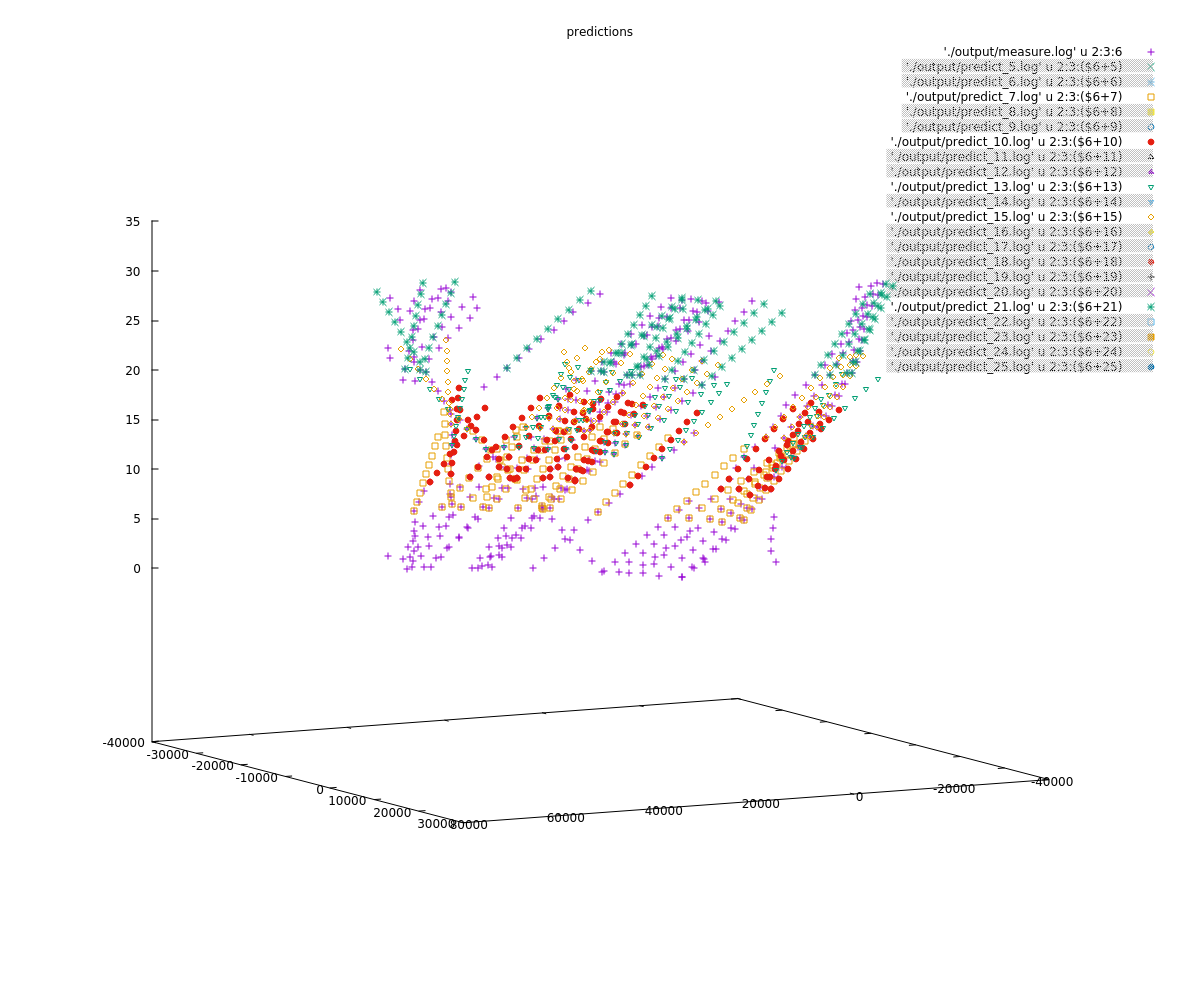
\includegraphics[width=\textwidth]{../graphs/prediction_data_2.png}
\end{figure}
\begin{figure}[H]
\caption{trial 3} 
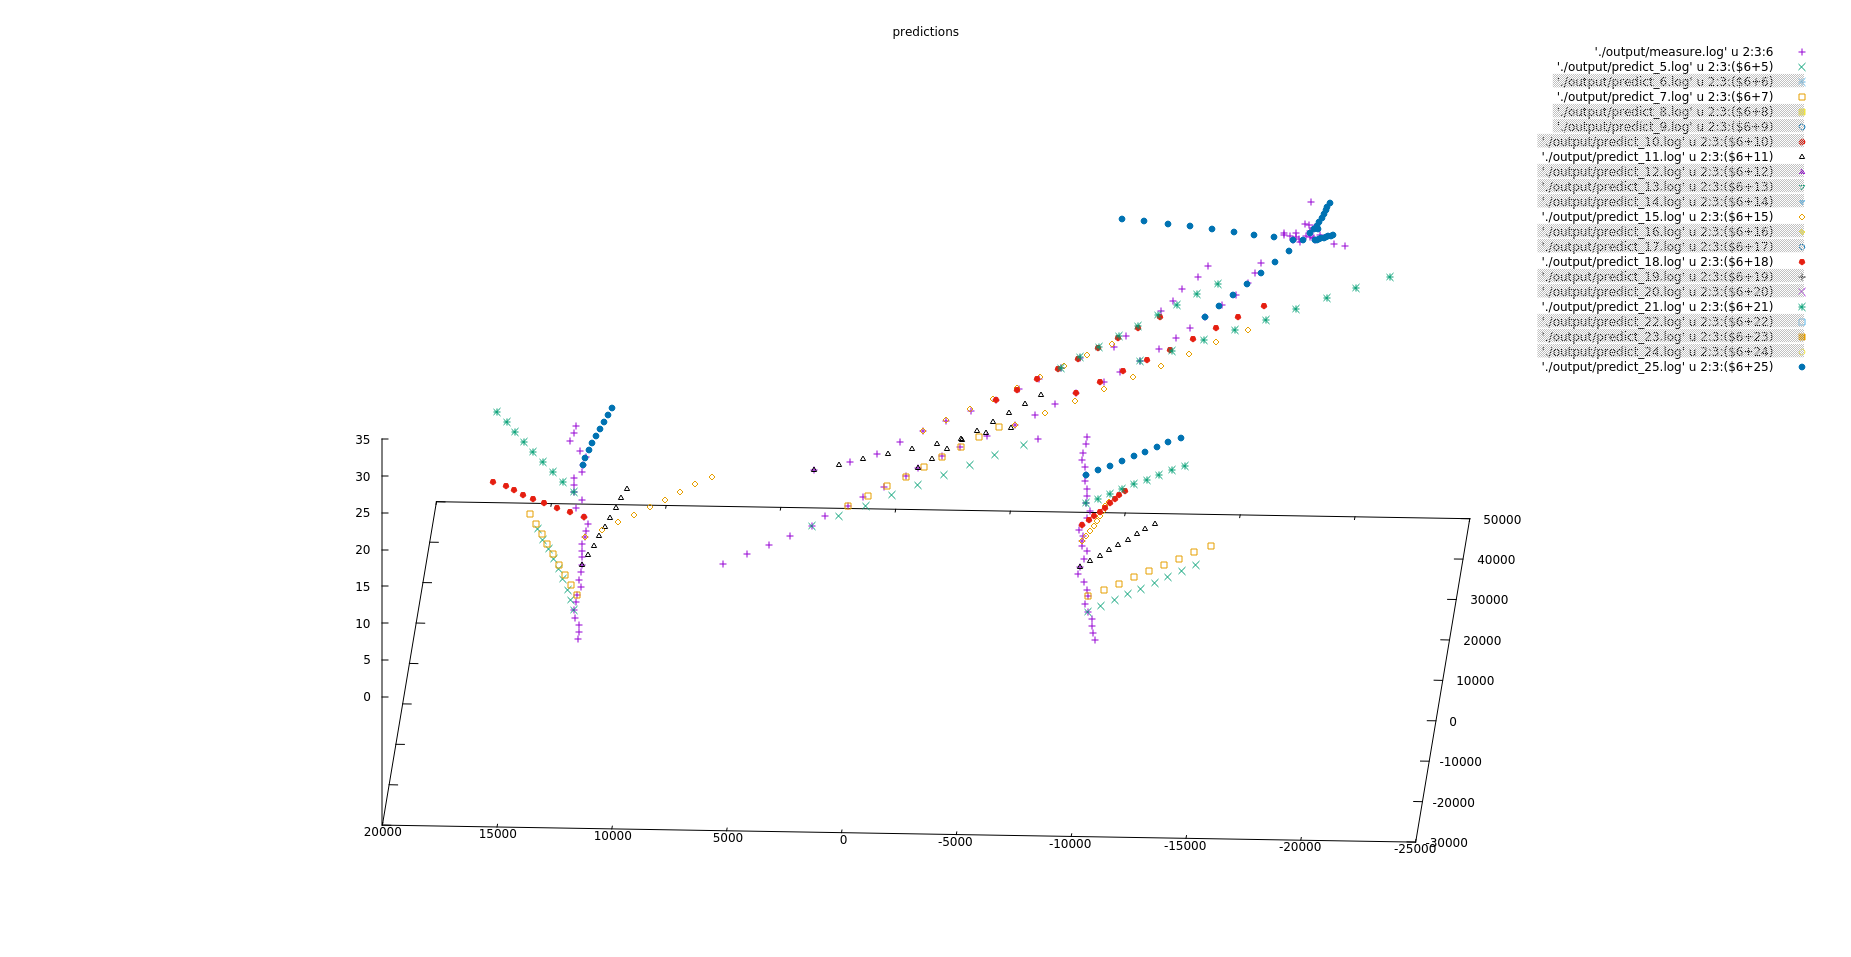
\includegraphics[width=\textwidth]{../graphs/prediction_data_3.png}
\end{figure}

\subsubsection{error profile}
\begin{figure}[H]
\caption{trial 2} 
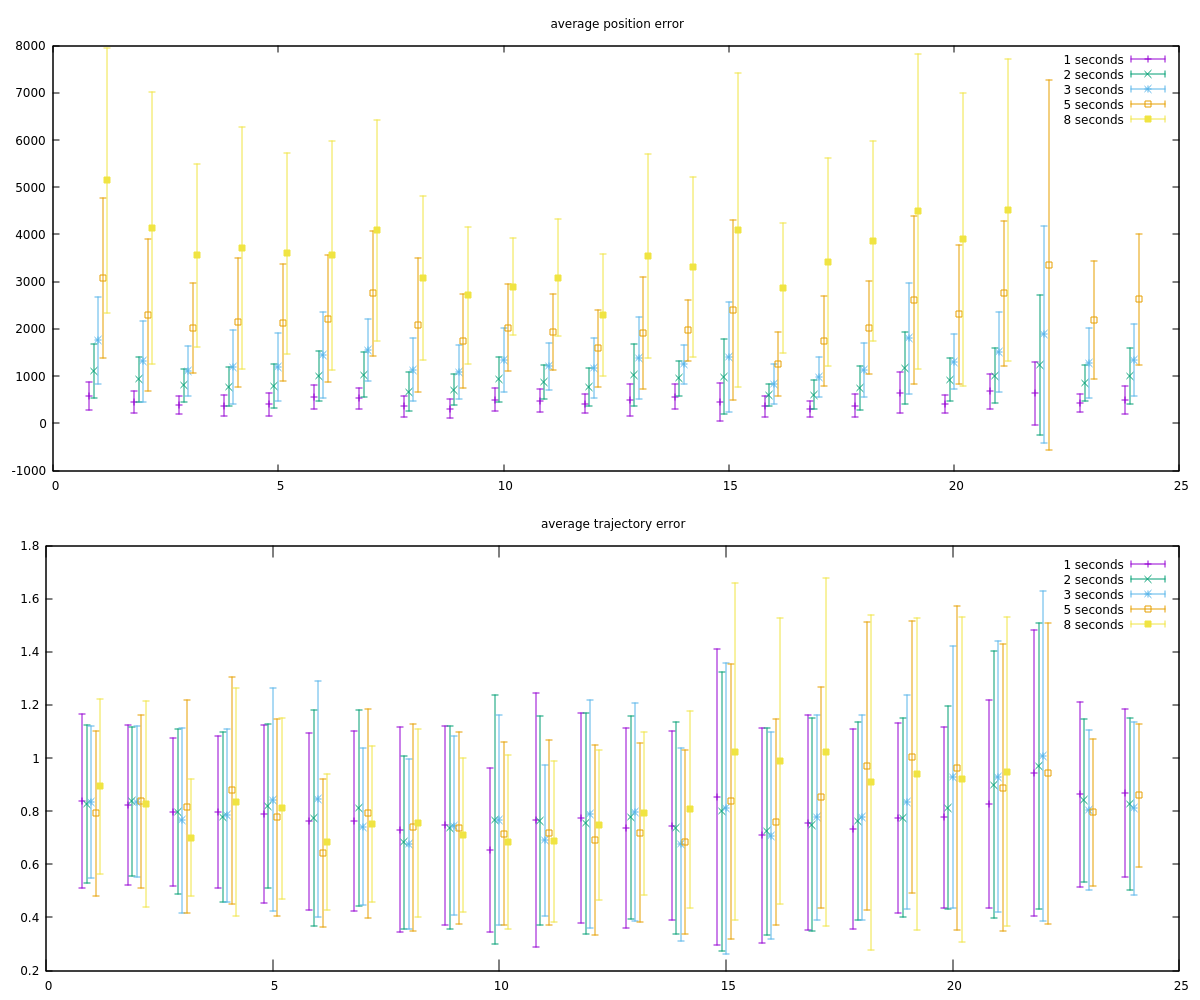
\includegraphics[width=\textwidth]{../graphs/error_profile2.png}
\end{figure}
\begin{figure}[H]
\caption{trial 3} 
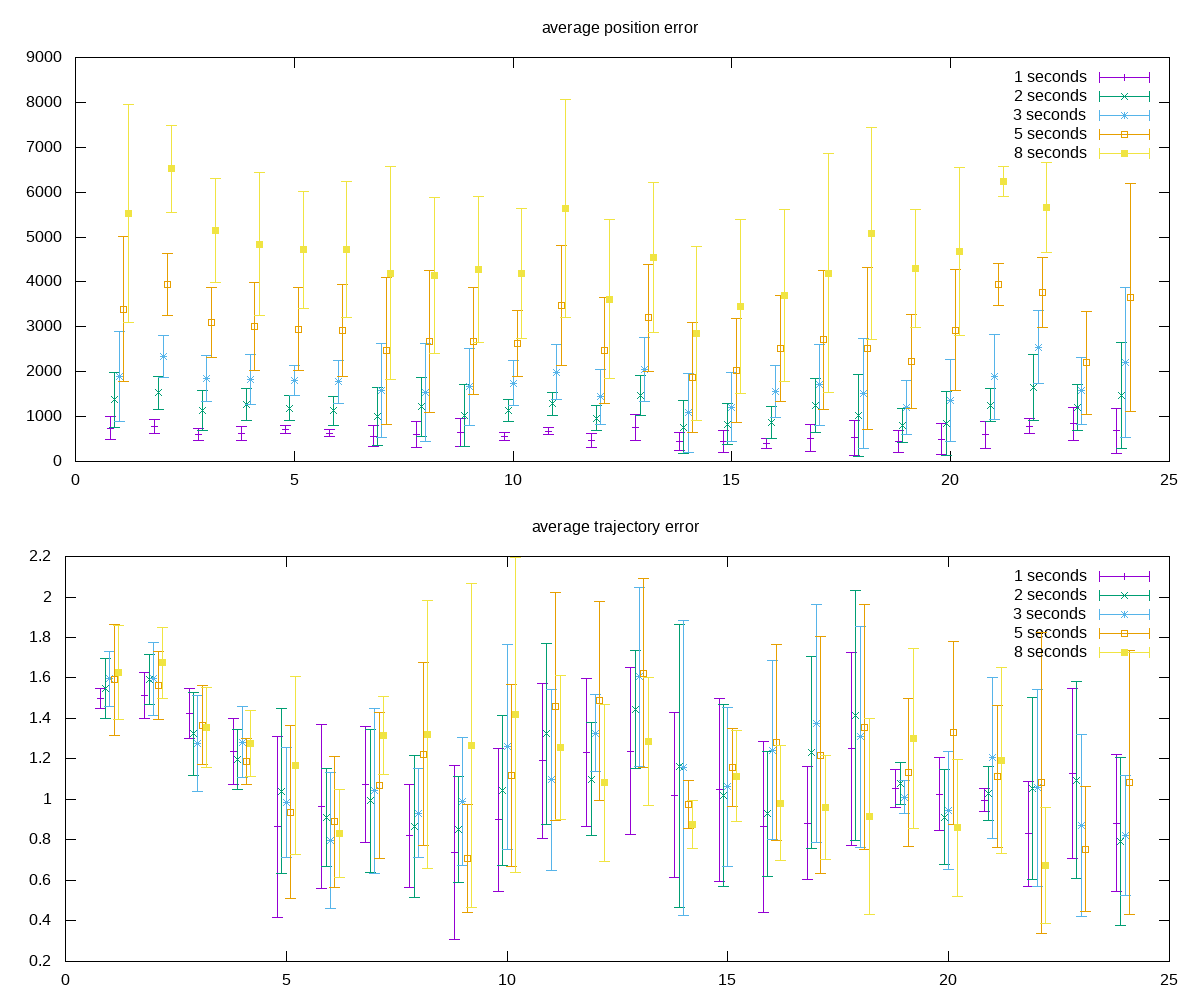
\includegraphics[width=\textwidth]{../graphs/error_profile3.png}
\end{figure}

\subsubsection{people tracks}
\begin{figure}[H]
\caption{trial 2} 
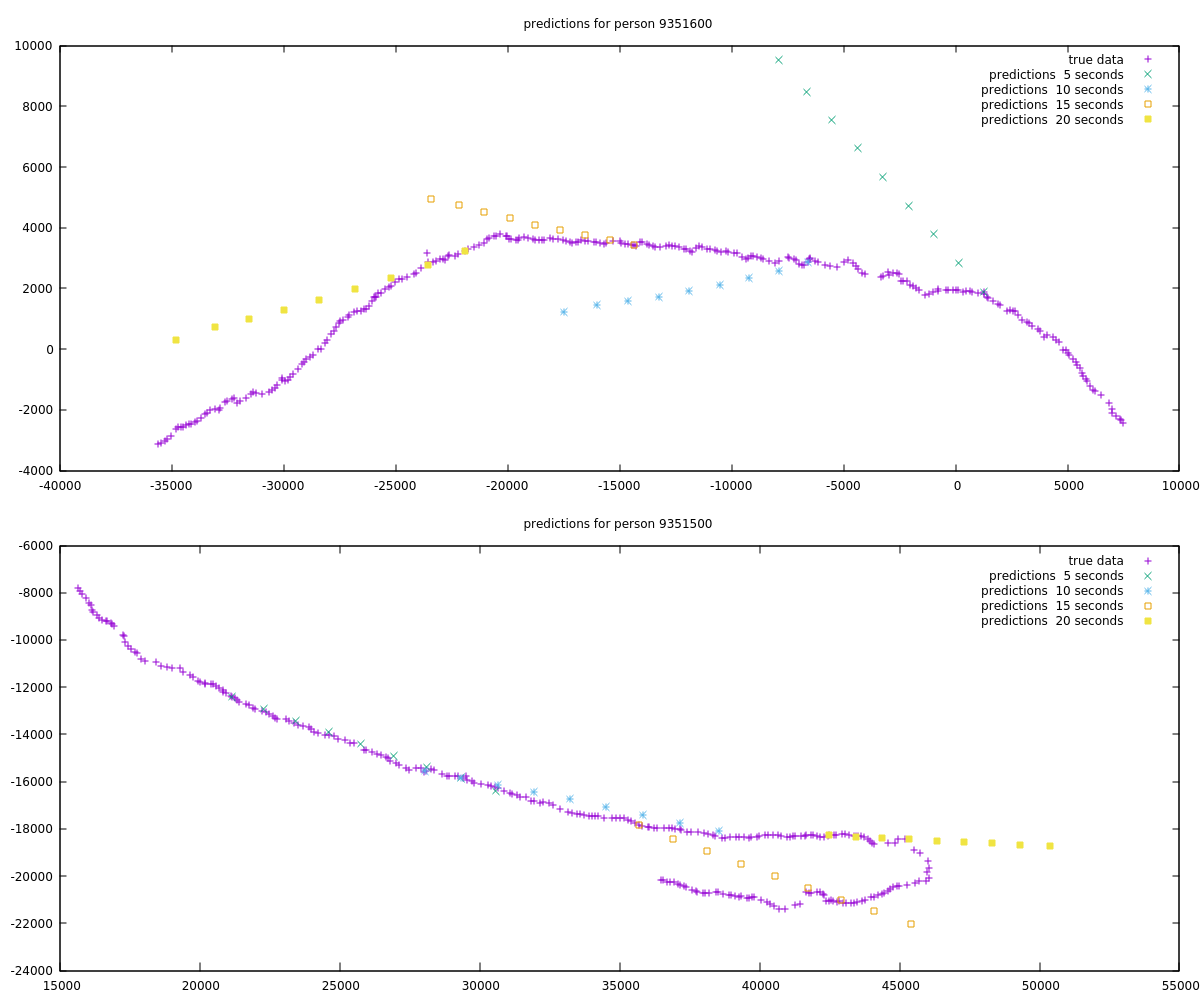
\includegraphics[width=\textwidth]{../graphs/person_tracks_2.png}
\end{figure}

\subsubsection{motion tracks}
\begin{figure}[H]
\caption{trial 2} 
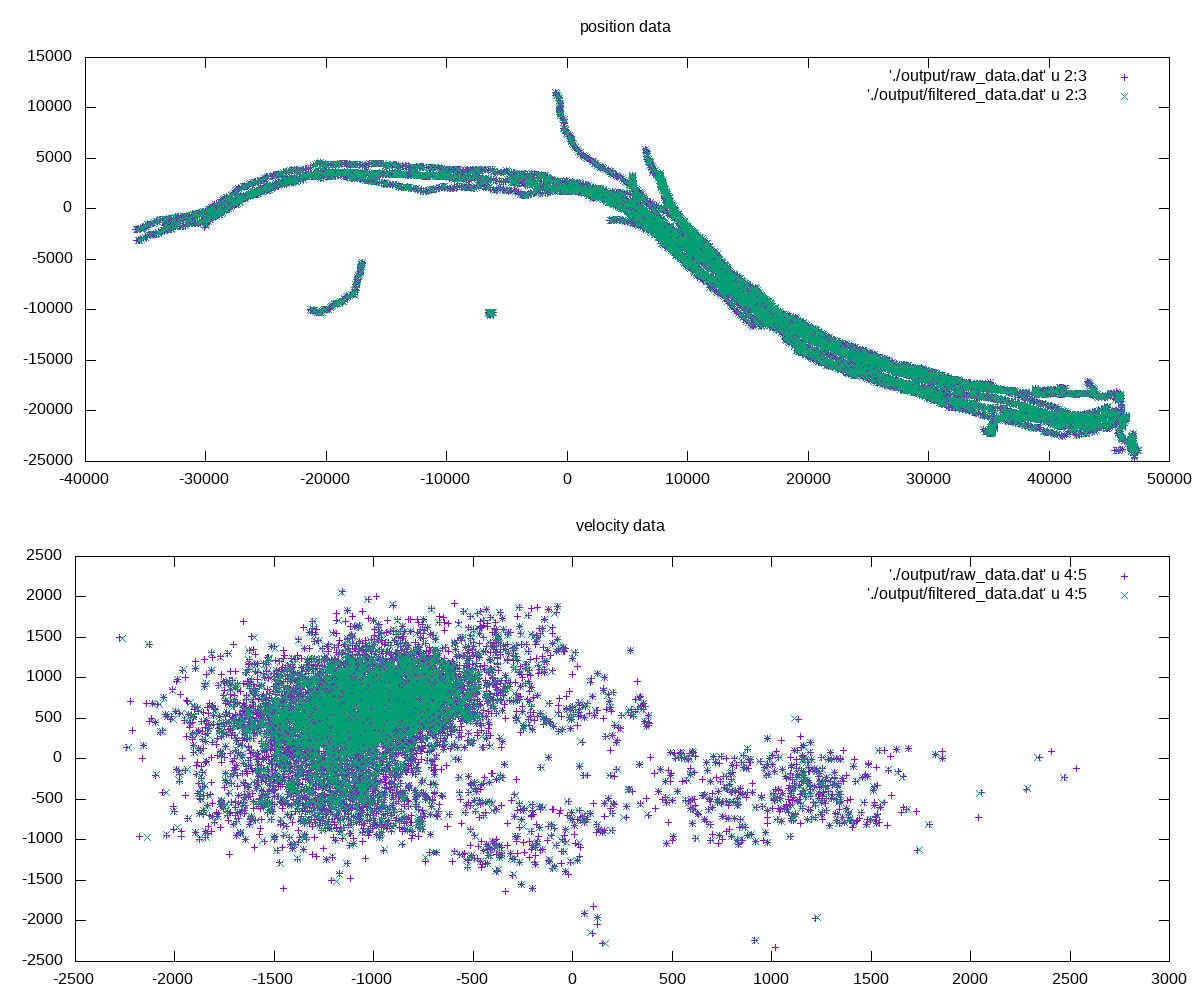
\includegraphics[width=\textwidth]{../graphs/raw_data_2.png}
\end{figure}
\begin{figure}[H]
\caption{trial 3} 
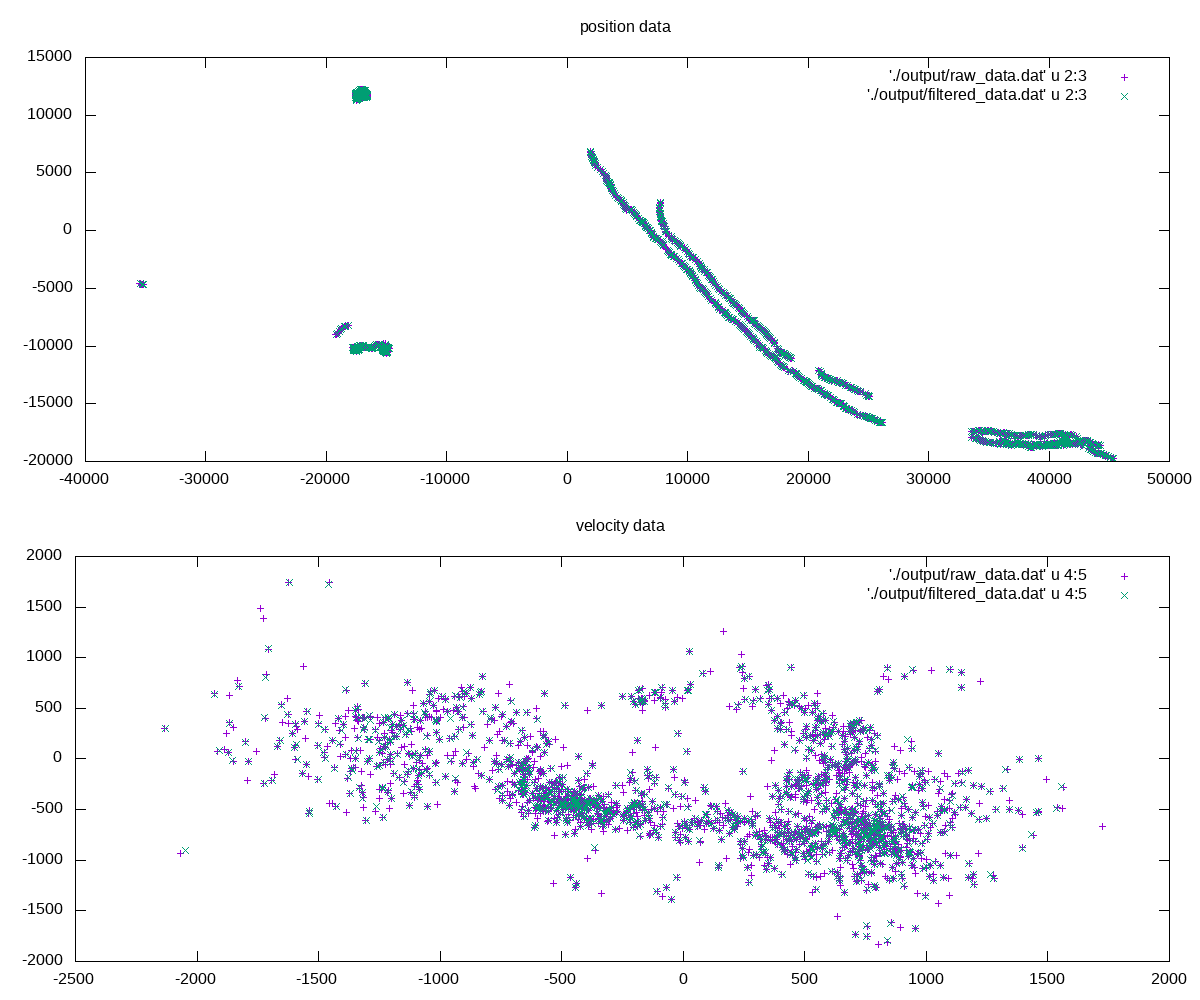
\includegraphics[width=\textwidth]{../graphs/raw_data_3.png}
\end{figure}

\subsection{Kalman Filter Full Evaluation Log}

\lstinputlisting[linerange={1-197}]{../output_one/prediction_report.txt}
\begin{center}
***
\end{center}
\lstinputlisting[linerange={1770-1936}]{../output_one/prediction_report.txt}
\begin{center}
***
\end{center}
\lstinputlisting[linerange={2429-2591}]{../output_one/prediction_report.txt}


\end{document}
